\input ../SlidePreamble
\input ../preamble

\begin{document}

{\Huge

  \centerline{\bf TTIC 31230, Fundamentals of Deep Learning}
  \bigskip
  \centerline{David McAllester, Fall 2023}
  \vfill
  \vfill
  \centerline{\bf Language Modeling}
  \vfill
  \centerline{\bf Recurrent Neural Networks}
  \vfill
  \centerline{\bf Machine Translation}
  \vfill
  \centerline{\bf The Transformer}
  \vfill
  \vfill

\slide{Language Modeling}

The recent progress on NLP benchmarks is due to pretraining on language modeling.

\vfill
Language modeling is based on unconditional cross-entropy minimiztion.

\vfill
$$\Phi^* = \argmin_\Phi \;E_{y \sim \pop}\;\left[-\ln P_\Phi(y)\right]$$

\vfill
In language modeling $y$ is a sentence (or fixed length block of text).

\slide{Language Modeling}

Let $V$ be some finite vocabulary of tokens.

\vfill
Each token is a character sequence that
can be used as a part of a rare word such a name in a foreign language.  Most English words
are a single token.

\vfill
Tokens typically do not cross word boundaries.

\vfill
We are interested in probability distributions over $V^*$ (the finite squanteces of tokens).

\slide{Language Modeling}

Let $\mathrm{Pop}$ be a population distribution over sequences of tokens.

\vfill
We want to train a model $P_\Phi(y)$ for token sequences $y$

\begin{eqnarray*}
\Phi^* & = & \argmin_\Phi \; E_{y \sim \mathrm{Pop}}\;\left[-\ln P_\Phi(y)\right]
\end{eqnarray*}

A structured object, such as a token sequence or an image, has an exponentially small probability.

\slide{Autoregressive Models}

An autoregressive model uses the chain rule to represent a distribution on sequences in terms of the conditional probability for each token given  the earlier tokens
tokens.

\vfill
$$P_\Phi(w_0, w_1, \cdots, w_T) = \prod_{t=0}^T\;P_\Phi(w_t\;|\;w_0,\ldots,w_{t-1})$$

\vfill
Modern language models are actually defining probability distributions on long sequences (thousands of tokens).

\slide{The end-of-squence token}

We want to define a probability distribution over sentence of different length.

\vfill
For this we require that each sentence is ``terminated'' with an end of sequence token {\tt <EOS>}.

\slide{Training}

$$P_\Phi(w_0, w_1, \cdots, w_T) = \prod_{t=0}^T\;P_\Phi(w_t\;|\;w_0,\ldots,w_{t-1})$$

\vfill
For training we need to compute the log loss on a training example.

\vfill
The log loss on a sequence is the sum of the log losses for each token generation.

\slide{Generation}
$$P_\Phi(w_0, w_1, \cdots, w_T) = \prod_{t=0}^T\;P_\Phi(w_t\;|\;w_0,\ldots,w_{t-1})$$

\vfill
We can generate from an autoregressive language model by generating one word at a time.

\vfill
To generate we sample from a probability distribution over the first word.  Once this word is generated
we compute a probability distribution for the second word and so on.

\slide{Word Embeddings}

Each word $w$ is associated with a vector $e(w)[I]$ called the embedding of word $w$.

\vfill
The matrix $e$ can be viewed as a dictionary assigning each word $w$ the vector $e(w)[I]$.

\slide{Recurrent Neural Network (RNN) Language Modeling}

\centerline{\includegraphics[width=3.5in]{\images/RNN}}
\centerline{{\large [Christopher Olah]}}

\vfill
A typical RNN neural language model has the form

$$P_\Phi(w_t\;|\;w_0,\cdots,w_{t-1}) = \softmax_{w_t} e(w_t)[I]h[t-1,I]$$

\slide{Vanilla RNNs}

\centerline{\includegraphics[width=3.5in]{\images/RNN}}
\centerline{{\large [Christopher Olah]}}

A Vanilla RNN uses two-input linear threshold units.

{\huge
\begin{eqnarray*}
{\color{red} h[t,j]}
& = & \sigma\left(W^{h,h}[j,I]{\color{red} h[t-1,I]} + W^{x,h}[j,K]{\color{red} x[t,K]} - B[j]\right) \\
\end{eqnarray*}
}

\slideplain{Exploding and Vanishing Gradients}

\vfill
If we avoid saturation of the activation functions then we get exponentially growing or shrinking eigenvectors of the weight matrix.

\vfill
Note that if the forward values are bounded by sigmoids or tanh then they cannot explode.

\vfill
However the gradients can still explode.

\slide{Exploding Gradients: Gradient Clipping}

\vfill
We can dampen the effect of exploding gradients by clipping them before applying SGD.

\vfill
$$W.\mathrm{grad'} = \left\{\begin{array}{l} W.\mathrm{grad} \;\;\;\mbox{if $||W.\mathrm{grad}|| \leq n_{\mathrm{max}}$} \\
                                                      \\ \\
                                                      n_{\mathrm{max}} \; W.\mathrm{grad} / ||W.\mathrm{grad}|| \;\; \mbox{otherwise}
\end{array} \right.$$

\vfill
See {\tt torch.nn.utils.clip\_grad\_norm}

\slide{Time as Depth}

\centerline{\includegraphics[width=3.5in]{\images/RNN}}
\centerline{{\large [Christopher Olah]}}

\vfill
We would like the RNN to {\color{red} remember and use} information from much earlier inputs.


\vfill
All the issues with depth now occur through time.

\vfill
However, for RNNs {\color{red} at each time step we use the same model parameters.}

\vfill
In CNNs {\color{red} at each layer uses its own model parameters.}

\slide{``Residual Connections'' Through Time}

\centerline{\includegraphics[width=3.5in]{\images/RNN}}
\centerline{{\large [Christopher Olah]}}

\vfill
We would like to have residual connections through time.

\vfill
However, we have to handle the fact that the same model parameters are used at every time step.


\slideplain{Gated RNNs}

\centerline{\includegraphics[width=3.5in]{\images/RNN}}
\centerline{{\large [Christopher Olah]}}

$$h[t,j] =  {\color{red} G_t[t,j]}h[t\!-\!1,j] + {\color{red} (1-G[t,j])}R[t,j]$$

\vfill
This is analogous to a residual connection.

\vfill
Rather than add the ``next layer'' $R[t,j]$ to the input $h[t\!-\!1,j]$ as in a residual connection, we take a convex combination determined by a computed ``gate'' $G[t,j] \in [0,1]$.

\slideplain{Update Gate RNN (UGRNN)}

{\huge
\begin{eqnarray*}
R[t,j] & = & \mathrm{tanh}\left(W^{h,R}[j,I]{\color{red} h[t\!-\!1,I]} + W^{x,R}[j,K]{\color{red} x[t,K]} - B^R[j]\right) \\
\\
G[t,j] & = & \sigma\left(W^{h,G}[j,I]{\color{red} h[t\!-\!1,I]} + W^{x,G}[j,K]{\color{red} x[t,K]} - B^R[j]\right) \\
\\
h[t,j] & = & {\color{red} G[t,j]}h[t\!-\!1,j] + {\color{red} (1-G[t,j])}R[t,j] \\
\\
{\color{red} \Phi} & {\color{red} =} & {\color{red} (W^{h,R},W^{x,R},B^R,W^{h,G},W^{x,G},B^G)}
\end{eqnarray*}
}
$$\mathrm{tanh}(x) \in (-1,1)\;\;\;\;\;\sigma(x) \in (0,1)$$

\slide{Hadamard product}

$$h[t,j] =  {\color{red} G[t,j]}h[t\!-\!1,j] + {\color{red} (1-G[t,j])}R[t,j]$$

\vfill
is sometimes written as

$$h[t,J] =  G[t,J]{\color{red} \odot} h[t\!-\!1,J] + (1-G[t,J]){\color{red} \odot} R[t,J]$$

\vfill
$\odot$ is the Hadamard product (componentwise product) on vectors.

\slide{Gated Recurrent Unity (GRU) by Cho et al. 2014}

\centerline{\includegraphics[width=4.0in]{\images/GRU}}

\slide{Long Short Term Memory (LSTM)}
\centerline{\includegraphics[width=3.5in]{\images/LSTM}}

\vfill
\centerline{[LSTM: Hochreiter\&Shmidhuber, 1997]}

\slide{UGRNN vs. GRUs vs. LSTMs}

[Collins, Dickstein and Sussulo 2016] found that the number of parameters is more important than the choice of RNN architectures.

\slide{bidirectional RNNS}

\centerline{\includegraphics[width = 6in]{\images/biRNN}}

\slide{Multi-Layer RNNs}

\centerline{\includegraphics[height = 4.0in]{\images/RNNstack}}

Modern versions would stack layers using residual connections.

\slide{Machine Translation}

$$w_0,\ldots,w_{T_{\mathrm{in}}} \Rightarrow \tilde{w}_0,\ldots,\tilde{w}_{T_{\mathrm{out}}}$$

\vfill
Translation is a {\bf sequence to sequence} (seq2seq) task.

\vfill
{\bf Sequence to Sequence Learning with Neural Networks}, Sutskever, Vinyals and Le, NeurIPS 2014, arXiv Sept 10, 2014.

\slide{Machine Translation}

\vfill
We define a model

\vfill
$$P_\Phi\left(\tilde{w}_0,\ldots,\tilde{w}_{T_{\mathrm{out}}}\;|\; w_0,\ldots,w_{T_{\mathrm{in}}}\right)$$

\vfill
\begin{eqnarray*}
\Phi^*  & = & \argmin_\Phi \; E_{\tuple{x,y} \sim \mathrm{Pop}} \; \left[-\ln P_\Phi(y|x)\right]
\end{eqnarray*}

\slide{Translation Using Thought Vectors}

\vfill
The final state of a {\bf right-to-left (backward)} RNN is viewed as a {\bf ``thought vector''} representation of the input sentence.

\vfill
We use the thought vector for the niput sentence as the initial hidden state of a {\bf left-to-right (forward)} RNN language model
generating the output sentence.

\vfill
Computing the input thought vector backward provides a good start to the forward generation of the output.

\slide{The Introduction of Attention}

{\bf Neural Machine Translation by Jointly Learning to {\color{red} Align} and Translate}
Dzmitry Bahdanau, Kyunghyun Cho, Yoshua Bengio, ICLR 2015 (arXiv Sept. 1, 2014)

\slide{Attention}

As we generate each word in the output translation we compute an attention over the input.

\vfill
Intuitively, we want to define an ``alignment'' between the words in the output and the words in the input.

\vfill
In modern terminology this is calles a ``cross attention'' --- one thing (the output) attending to a different thing (the input).

\vfill
This is different from the ``self attention'' used in transformers.

\slide{Encoder-Decoder Models with Cross-Attention}

Let $h_{\mathrm{thought}}$ be the thought vector for the input sentence.

\vfill
Let $h_{\mathrm{in}}(t_{\mathrm{in}})$ be a sequence of vectors generated by the encoder for the sequence of input words.

\vfill
Let $h_\mathrm{out}(t_\mathrm{out})$ be a thought vector for the first $t_\mathrm{out}$ words in the output sentence.

\vfill
{\huge
$$\begin{array}{rrcl}
  \mathrm{Attention}\; & {\color{red} \alpha[t_\mathrm{out},t_{\mathrm{in}}]} & =& \softmax_{t_\mathrm{in}} \;e(w_{t_\mathrm{out}})[N]\;h_\mathrm{in}(t_\mathrm{in})[N] \\
   \\
   \mathrm{Weighted\; Sum:} & \tilde{h}_\mathrm{out}(t_\mathrm{out}) & = & {\color{red} \alpha[t_\mathrm{out},T_{\mathrm{in}}]}\;h_\mathrm{in}(T_{\mathrm{in}}) \\
  \\
  \mathrm{generate:} & w_\mathrm{t_\mathrm{out} + 1} & \sim & P_\Phi(w_{t_\mathrm{out}+1}\;|h_\mathrm{thought},
  h_\mathrm{out}(t_\mathrm{out}),
  \tilde{h}_\mathrm{out}(t_\mathrm{out}))
  \end{array}$$
}

\slide{Cross Attention in Image Captioning}
We can treat image captioning as translating an image into a caption.

\vfill
In translation with attention involves an attention over the input aligning output words with positions in the input.

\vfill
For each output word we get an attention over the image positions.

\slide{Attention in Image Captioning}

\centerline{\includegraphics[height = 4.8in]{\images/AttentionInCaptioning1}}
\centerline{\Large Xu et al. ICML 2015}

\slide{The Transformer: Self Attention}

Attention is All You Need, Vaswani et al., June 2017

\vfill
We replace the RNNs with self attention.

\vfill
For the encoder we will have a ``residual stack'' $h_{0,\mathrm{in}}(t_\mathrm{in}),\ldots,h_{N,\mathrm{in}}(t_\mathrm{in})$.

\vfill
Set $h_{0,\mathrm{in}}(t_\mathrm{in}) = e(w_{t_\mathrm{in}});\mathrm{pos}(t_\mathrm{t_\mathrm{in}})$.

\vfill
Here semicolon denotes vector concatenation and $\mathrm{pos}(t_\mathrm{in})$ is a ``position encoding'' for the position $t$.

\slide{The Residual stack}
\centerline{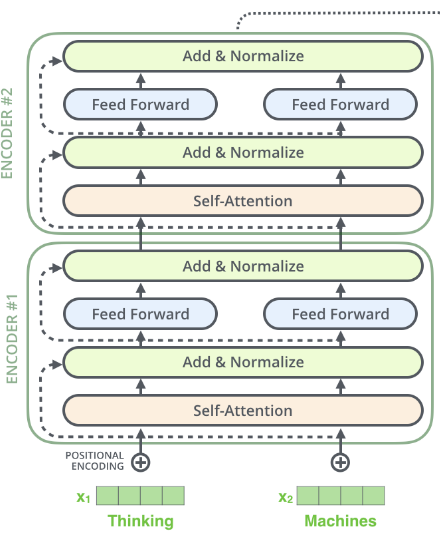
\includegraphics[height=5.0in]{\images/transformer}}


\slide{Parallel Layer Computation}

However, in the transformer we can compute the layer $L_{\ell+1}[T,J]$ from $L_\ell[T,J]$ in parallel.

\vfill
This is an important difference from RNNs which compute sequentially over time.

\vfill
In this respect the transformer is more similar to a CNN than to an RNN.

\slide{Self-Attention}

The fundamental innovation of the transformer is the self-attention layer.

\vfill
For each position $t$ in the sequence we compute an attention over the other positions in the sequence.

\slide{Transformer Heads}

There is an intuitive analogy between the Transformer's self attention and a dependency parse tree.

\vfill
In a dependency parse cibsists if edges between words labeled with grammatical roles such as ``subject-of'' or ``object-of''.

\vfill
The self attention layers of the transformer we have ``heads'' which can be viewed as labels for dependency edges.

\vfill
Self attention constructs a tensor $\alpha[k,t_1,t_2]$ --- the strength of the attention weight (edge weight)
from $t_1$ to $t_2$ with head (label) $k$.

\slide{Query-Key Attention}

For each head $k$ and position $t$ we compute a key vector and a query vector with dimension $I$ typically smaller than dimension $J$.

{\huge
\begin{eqnarray*}
\mathrm{Query}_{\ell+1}[k_\mathrm{head},t,i] & = & W^\mathrm{querry}_{\ell+1}[k_\mathrm{head},i,J]L_\ell[t,J] \\
\\
\mathrm{Key}_{\ell+1}[k_\mathrm{head},t,i] & = &  W^\mathrm{key}_{\ell+1}[k_\mathrm{head},i,J]L_\ell[t,J] \\
\\
\alpha_{\ell+1}[k_\mathrm{head},t_1,t_2] & = & \softmax_{t_2}\; \frac{1}{\sqrt{I}}\;\mathrm{Query}_{\ell+1}[k_\mathrm{head},t_1,I]\mathrm{Key}_{\ell+1}[k,t_2,I]
\end{eqnarray*}
}

\slide{Computing the Self-Attention Layer}
      
\begin{eqnarray*}
\mathrm{Value}_{\ell+1}[k_\mathrm{head},t,i] & = & W^V_{\ell+1}[k_\mathrm{head},i,J]L_\ell[t,J] \\
\\
\tilde{h}_{\ell+1}[k_\mathrm{head},t,i] & = & \alpha[k_\mathrm{head},t,T]\mathrm{Value}[k_\mathrm{head},T,i] \\
\\
\hat{h}_{\ell+1}[t,C] & = & \tilde{h}_{\ell+1}[0,t,I];\cdots;\tilde{h}_{\ell+1}[K_\mathrm{head}-1,t,I] \\
\\
L^{SA}_{\ell+1}[t,j] & = & W^0_{\ell+1}[j,C]\hat{h}_{\ell+1}[t,C]
\end{eqnarray*}

\vfill
Here semicolon denotes vector concatenation.

\slide{Attention in Image Captioning}

We have now defined the self-attention layer.
\vfill
\centerline{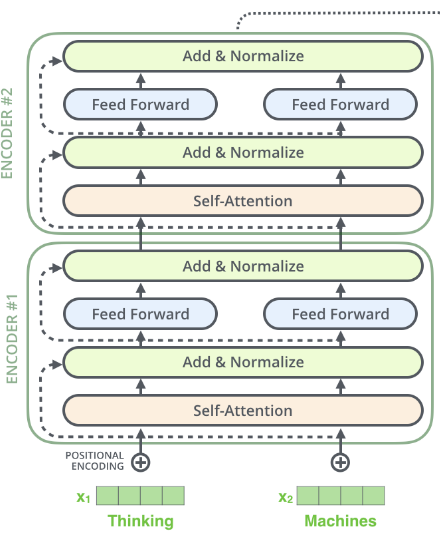
\includegraphics[height=4.0in]{\images/transformer}}

\slide{Feed-Forward Layers}

The feed-forward layers apply a two-level multi-layer perceptron (MLP) to the vector at each time position independently.

\vfill

\begin{eqnarray*}
h_{\ell+1}[t,i] & = & \mathrm{ReLU}(W^{\mathrm{FF1}}_{\ell+1}[i,J]\;L_\ell[t,J] - B^{\mathrm{FF1}}_{\ell+1}[i]) \\
\\
L_{\ell+1}[t,j] & = & W^{\mathrm{FF2}}_{\ell+1}[j,I]\;h_{\ell+1}[t,I] - B^\mathrm{FF2}_{\ell+1}[j]
\end{eqnarray*}

\slide{The Transformer}

\centerline{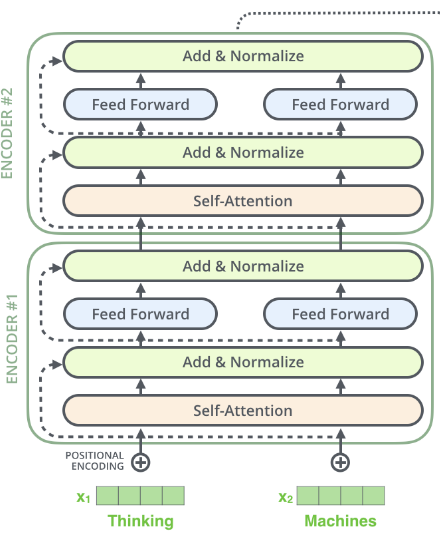
\includegraphics[height=5.0in]{\images/transformer}}

\slide{END}
}
\end{document}
